\documentclass{article}
\usepackage[utf8]{inputenc}
\usepackage[brazilian]{babel}
\usepackage{outlines}
\usepackage{graphicx}
\usepackage{indentfirst}
\usepackage{datetime}
\setlength{\parskip}{.5em}
\usepackage{enumitem}
\setlist{nosep}
\usepackage[section]{placeins}
\def\tam{0.6}
\usepackage[all]{nowidow}
\nowidow
\noclub
\usepackage[scale=1.5]{ccicons}
\usepackage{authblk}
\usepackage{hyperref}
\title{Dicas para Provas de Aula}
\author{Geraldo Xexéo}
\affil{\url{xexeo@ufrj.br} \\
\url{http://xexeo.net}}
\date{\ccbyncsa\  - \today}

\begin{document}


\maketitle

\begin{abstract}
    Este documento apresenta dicas para provas de aula de concurso para universidades públicas, que devem ser usadas tanto em concursos para professor adjunto quanto para professor substituto.
\end{abstract}




\section{Dicas gerais}



A prova de aula é uma \textbf{aula}, que deve ser \textbf{dada para a banca como se ela fosse uma turma comum} da instituição para a qual você concorre. Na prática, é quase um teatro. Aviso isso antes de tudo, que parece algo básico, porque já vi um candidato dar uma palestra explicando  como seria sua aula, devido a prática de avaliação de uma instituição privada.

Pelo regulamento, você não pode ultrapassar o prazo dado para a aula, em torno de 50 minutos. Você \textbf{deve usar exatamente o tempo destinado à prova de aula}, nem mais, o que não será permitido pela banca, nem menos. Para isso, o ideal é preparar uma aula um pouco menor, já que costumamos ser otismistas quanto ao tempo necessário para dar uma aula, porém com exercícios ou outras atividades no fim, que possam ser feitos detalhadamente, se sobrar tempo, ou ser repassadas rapidamente como ``dever de casa''. Desse jeito, você pode atrasar um pouco sem se preocupar muito, utilizando essa margem para explicações e exemplos melhores que descobriu ou lembrou naquele instante. Isso será compensado mais tarde reduzindo a atenção dada aos exercícios.Por outro lado, você também pode usar esses exercícios para usar um tempo que tenha sobrado. Isto pode ser feito fazendo o exercício ou dando dicas.

A aula deve estar no contexto de um curso. Você deve procurar a ementa do curso para o qual estaria dando aula e, no início da aula, contextualizar a mesma dentro de um curso imaginário que cumpra essa ementa. Por exemplo, você pode mostrar a lista de assuntos do curso e indicar em que aula está. Deve também falar um pouco sobre a última aula e como ela e a aula atual se relacionam.

O \textbf{português} utilizado será determinante na sua pontuação. Erros de português no material impresso são graves, e erros de fala são normalmente percebidos e causam perda de pontos. Muito cuidado com a concordância verbal e com defeitos de linguagem que sabemos que temos, mas não nos preocupamos na fala coloquial. Pessoas de outros estados, diferentes do local do concurso, devem tomar cuidado com expressões locais que não serão compreendidas pela banca.

Se você já deu aulas, deve tentar fazer ou simular tudo que faz com seus alunos normalmente, principalmente o que tem sucesso, e o que gostaria de fazer. Por exemplo, criar um \textit{Moodle} ou um \textit{Google Classroom} para a turma. Na aula, você deve então indicar em que parte do \textit{site} está sua aula, como os alunos podem baixar e que exercícios devem fazer ou entregar.

A prova de aula, como diz o nome, é sobre como você dá aula. Use sua experiência. Não se preocupe em estar apresentando a aula para uma banca de professores reconhecidos ou exigentes. Não é uma apresentação de trabalho em congresso, você deve dar a aula  como se fosse para sua turma, porém com um cuidado adicional de não ser tão informal ao ponto de cometer erros de comportamento ou de português.

Ao preparar a aula, lembre-se que a banca não só já conhece o assunto como pode ser especialista nele, mas os supostos alunos, não. Eu recomendo procurar fontes sólidas e básicas, ter cuidado com a profundidade em que o tema é abordado e buscar a facilitação do aprendizado, através de exemplos e exercícios.

Se o tema for muito amplo, você tem duas opções: dar uma aula introdutória ou escolher um sub-tema. A validade de escolher um sub-tema pode ser perguntada a banca, que pode ou não responder. Se a banca não responder, sugiro escolher a aula introdutória. Nessa aula, no final você deve indicar como as próximas aulas vão se aprofundar no tema.

\section{Material para a aula}

Você deve tentar levar todo o material possível para a aula.

Caso vá usar um computador para fazer a apresentação e possua um notebook, deve tentar apresentar com seu equipamento, já que isso diminuirá a chance de problemas por não saber onde está algum software necessário ou com versões do mesmo.

Se pretende usar giz ou quadro branco, deve leva seus kits coloridos e apagadores, pois não necessariamente terá todo o material que deseja disponível na hora.

Sempre traga a aula, em vários formatos, em um drive USB, caso seu computador, ou outro, falhe, ou a rede não funcione.

Se não for usar seu computador, salve sua aula não só no formato original, mas também em formatos alternativos. Não deixe de ter a apresentação em formato .pdf, que transita bem entre os vários sistemas operacionais.

Não esqueça de, ao criar os arquivos .ppt, .pptx ou .pdf, incluir as fontes dentro deles.

Se possível, leve um ``passador de slides'', aquele controle remoto que permite passar os slides a distância.

\section{Slides}

Esta seção foi ampliada no documento ``Dicas de Como Fazer Slides Acadêmicos'', que pode ser encontrado em:

\url{https://github.com/xexeo/DicasSlidesAcademicos}.

Recomendo o uso de slides, como chamarei aqui a apresentação tipicamente feita com \textit{Power Point}. Eles devem estar incluídos na lista de recursos didáticos e devem ser entregues, de forma impressa, para a banca, indicando o fato deles estarem disponíveis em algum site ou \textit{Course Management System - CMS}, como o \textit{Moodle}.

A média de slides como os que apresento neste texto é de 2 a 3 minutos, porém alguns slides demoram muito pouco, porque são apenas marcos para indicar em que ponto da aula estamos.

\textbf{Todos seus slides devem estar em português}, a não ser que seja outra a exigência do concurso, o material, como um todo, deve ser original. Tudo que não for original deve ter uma citação. A consideração com os alunos também é avaliada, tanto quanto a suposta ``preguiça'' de não fazer o material próprio. Não apresente um material pré-pronto, como o disponível para acompanhar um livro. Faça o seu material, dite seu próprio ritmo. Nada impede, porém, que se inspire em outras aulas disponíveis na rede.

O ideal seria você criar do zero todas as imagens. Claro que algumas imagens não podem ser originais, como fotos. Por exemplo, no slide \ref{fig:crisis} eu mostro uma caricatura original em inglês, da época da Crise do Software. No concurso, na verdade, sempre há  margem de usar imagens de outros autores, porque o tempo é curto. É necessário, porém, citar a fonte.

\begin{figure}[!htb]
    \centering
    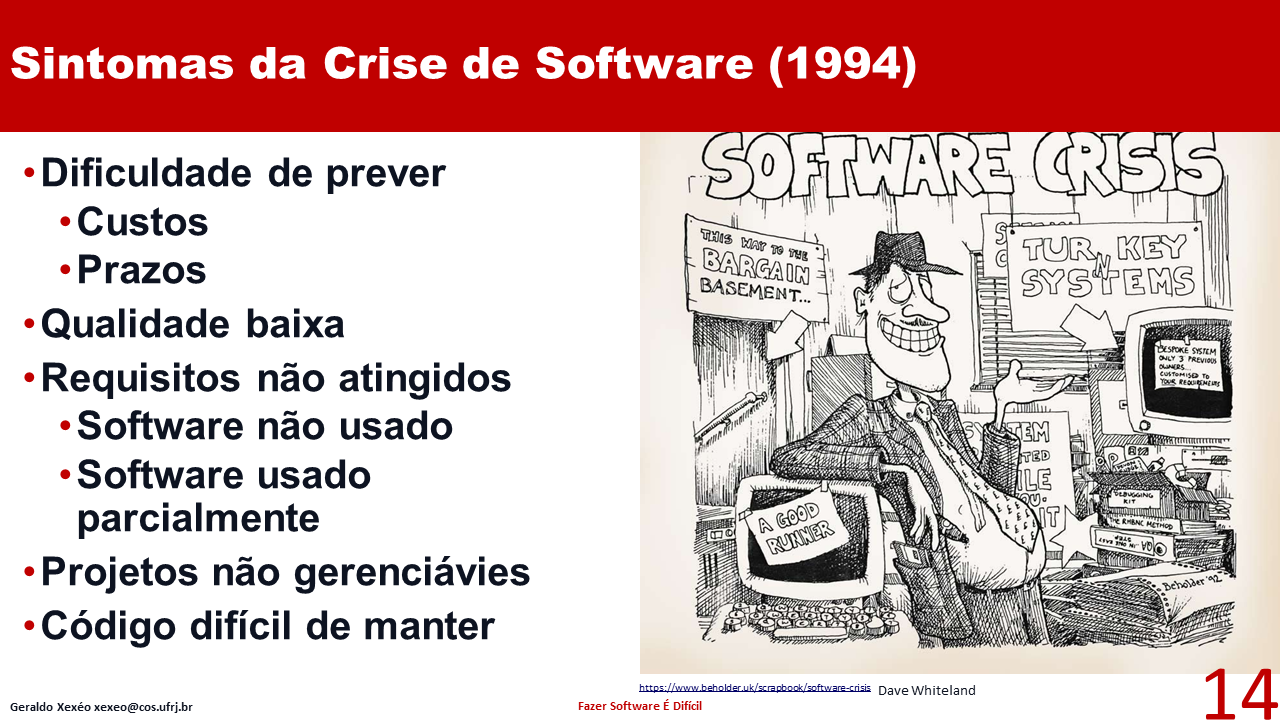
\includegraphics[width=\tam\linewidth]{imagens/crisis.png}
    \caption{Slide mostrando uma imagem original, onde a língua original é permitida.}
    \label{fig:crisis}
\end{figure}

Deve-se evitar slides que falam muito sobre algo sem mostrar como é feito. Há algum tempo eu costumo dar \textit{spoilers} mostrando as coisas antes de explicar o que saõ, sobre que estou falando, mas só mostrar uma imagem no mesmo slide em que se explica algo ajuda muito.

A ideia aqui é não confundir a banca, ou os possíveis alunos, e indicar para onde estamos indo. Isso também pode ser feito com texto ou com matemática. Por exemplo, em uma sequência de slides onde se prova um teorema ou se calcula algo podemos sempre mostrar nosso objetivo.

A Figura \ref{fig:teximag} mostra a explicação de um ator em um Diagrama de Caso de Uso sendo feita, ao mesmo tempo, de forma conceitual e gráfica. Seria ainda melhor se houvesse um pequeno exemplo de uso.

\begin{figure}[hbt]
    \centering
    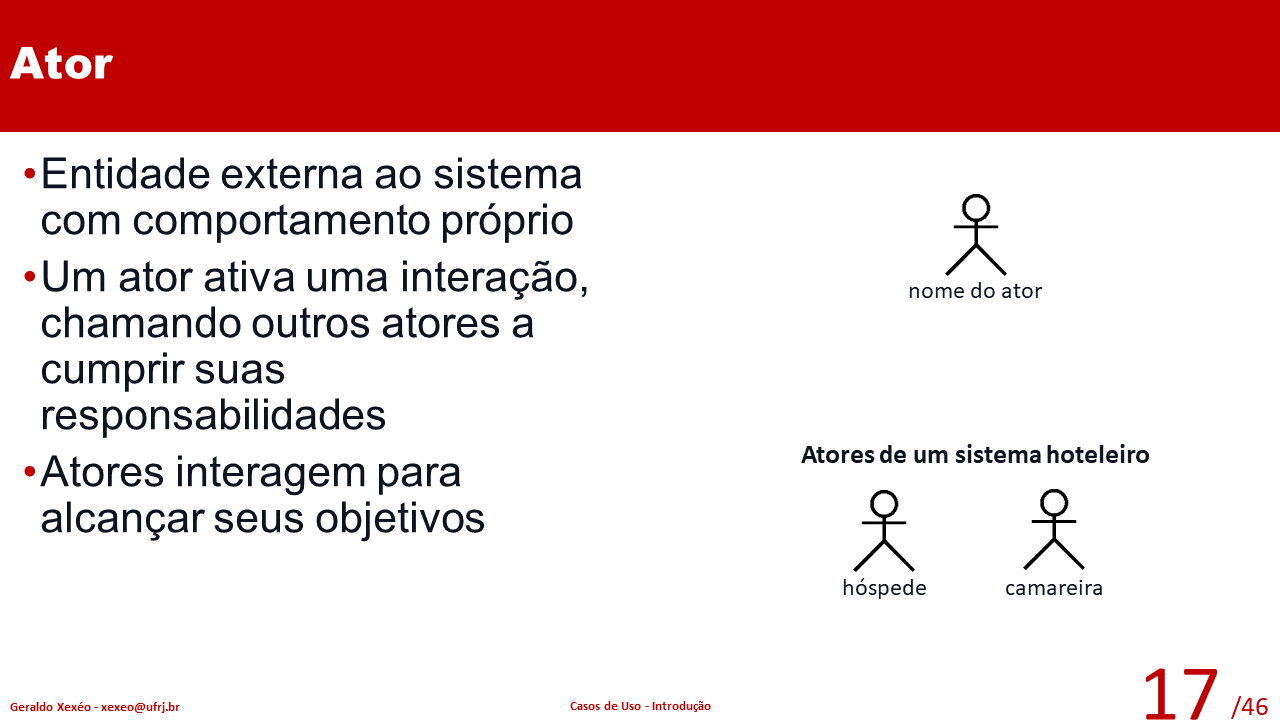
\includegraphics[width=\tam\linewidth]{imagens/slidecomimage.png}
    \caption{Slide com texto e imagem}
    \label{fig:teximag}
\end{figure}

Você, porém, não deve usar apenas os slides ao dar a aula, devendo também usar o quadro branco ou negro, por exemplo, para resolver um problema ou mostrar alguma ideia adicional. Esse recurso, o quadro branco ou negro, deve estar na lista de recursos.


\subsection{Regras essenciais sobre os slides}

Os slides \textbf{devem ser numerados} e conter em cada slide o número total de slides, possivelmente no formato ``slide/total'', como em ``4/40''. Eu uso número bem grandes e recomendo usá-los.

Todo slide deve ter um \textbf{título único}. Algumas pessoas gostam de usar um título de seção e um subtítulo que diz o que realmente o slide diz, mas isso faz com que cada slide pareça ser o mesmo que o outro e eu discordo dessa abordagem. A Figura \ref{fig:coppe} mostra um slide seguindo essa regra. A Figura \ref{fig:meio} mostra um slide que tem todas as seções identificadas em seu cabeçalho, sendo que a seção atual está com ênfase. Nesse caso, o título principal ainda é o título do slide. Isso pode ser feito automaticamente em alguns estilos para \texttt{beamer} no \LaTeX.

Todos os slides devem identificar a aula, o autor, incluindo o e-mail. Eu coloco isso no rodapé, o que é realmente o lugar para colocá-los no \textit{Power Point}. A instituição pode ser indicada através de um logo, como o slide da Figura \ref{fig:coppe}\footnote{Os slides vermelhos não têm a identificação da instituição porque são usados em mais de um curso}.

\begin{figure}[htb]
    \centering
    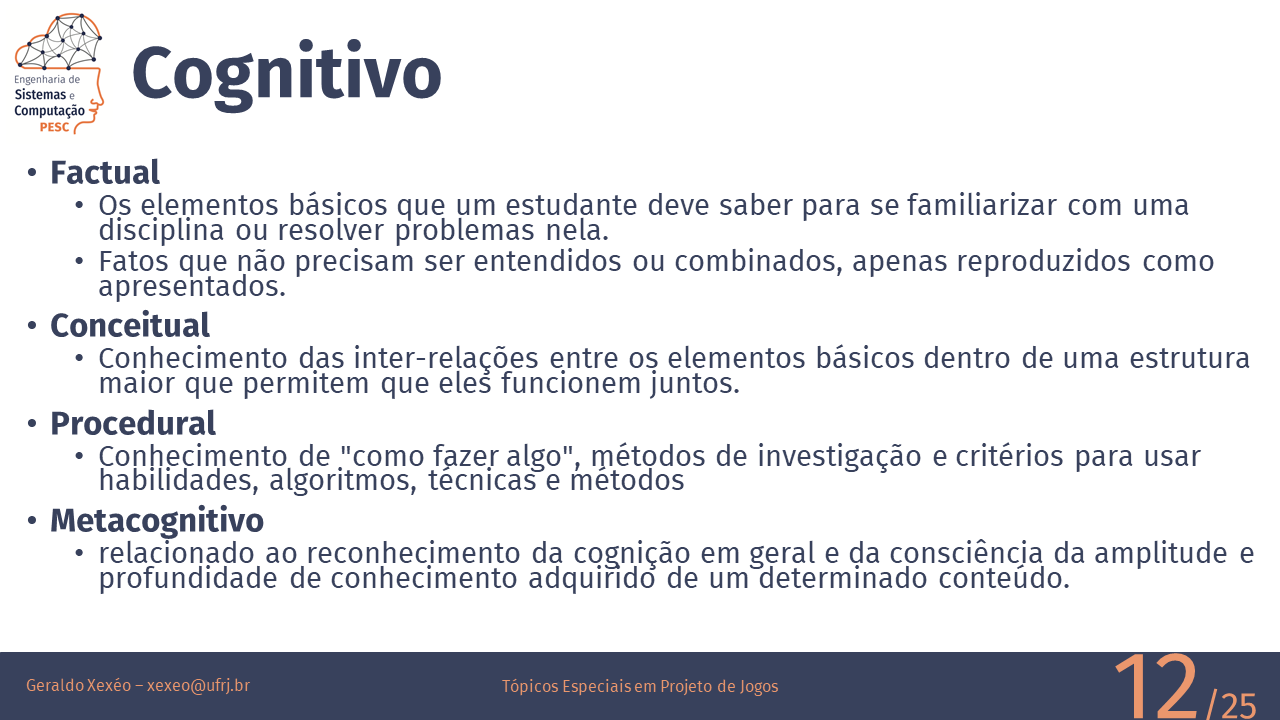
\includegraphics[width=\tam\linewidth]{imagens/slideexemplotepj.png}
    \caption{Um slide com logo, um título único, identificação, número do slide e número total de slides}
    \label{fig:coppe}
\end{figure}

Use fontes ``limpas'', não rebuscadas, e \textbf{sem-serifa}\footnote{Serifas são as pontinhas que existem em algumas fontes. Elas estão bem visíveis no S da palavra ``slides'' desta seção.}, como Arial ou Calibri, e \textbf{corpos grandes}, 32 pts, por exemplo. Os slides das Figuras \ref{fig:coppe} e \ref{fig:teximag} seguem essa regra. Já o slide da figura \ref{fig:formulas} usa um tamanho menor para o corpo das fórmulas. Lembre que a banca, ao invés dos alunos, é mais velha e pode ter dificuldades de visão.

A melhor estratégia para o estilo dos slides de aula são o fundo branco, letras escuras, e cores para ressaltar. Isso se adequa bem tanto a salas bem iluminadas quanto a salas escuras, para todo tipo de projetor. A Figura \ref{fig:teximag}, apesar de usar o forte grená, me parece bastante adequada. As outras figuras  mostram outros modelos que eu uso e sinto adequados para uma aula. As cores azuis e cinzas, porém, são mais ``fracas'' e podem levar a um pouco de monotonia.

Slides ``divertidos'', como os que estão resumidos\footnote{Esses slides foram encontrados em     \url{https://unblast.com/funtastic-free-powerpoint-presentation-template-ppt/}
    } na Figura \ref{fig:fun} vão criar uma carga cognitiva muito grande em uma apresentação e podem incomodar membros da banca. Já vi isso acontecer. Mas isso não quer dizer que não possam ser usados em um ou outro slide, como marcos de início de seção ou outra alternativa de menor impacto que usá-los em toda aula.

\begin{figure}[hbt]
    \centering
    
\includegraphics[width=\tam\linewidth]{imagens/funslide.jpg}
    \caption{Exemplos de slides divertidos.
    (Fonte: unblast.com) }
    \label{fig:fun}
\end{figure}


É importante variar o estilo do slide. Isso é bem fácil no \textit{Power Point}, porém é mais difícil no \texttt{beamer}, por exemplo. A Figura \ref{fig:man} mostra um slide bem diferente do que os apresentados normalmente, mas ainda em um formato ``retangular''. Use os formatos para tirar a monotonia da aula. Use também animações nos slides, mas cuidado com as transições entre os slides, que devem ser usadas muito parcimoniosamente, porque quebram a atenção.

\begin{figure}[htb]
    \centering
    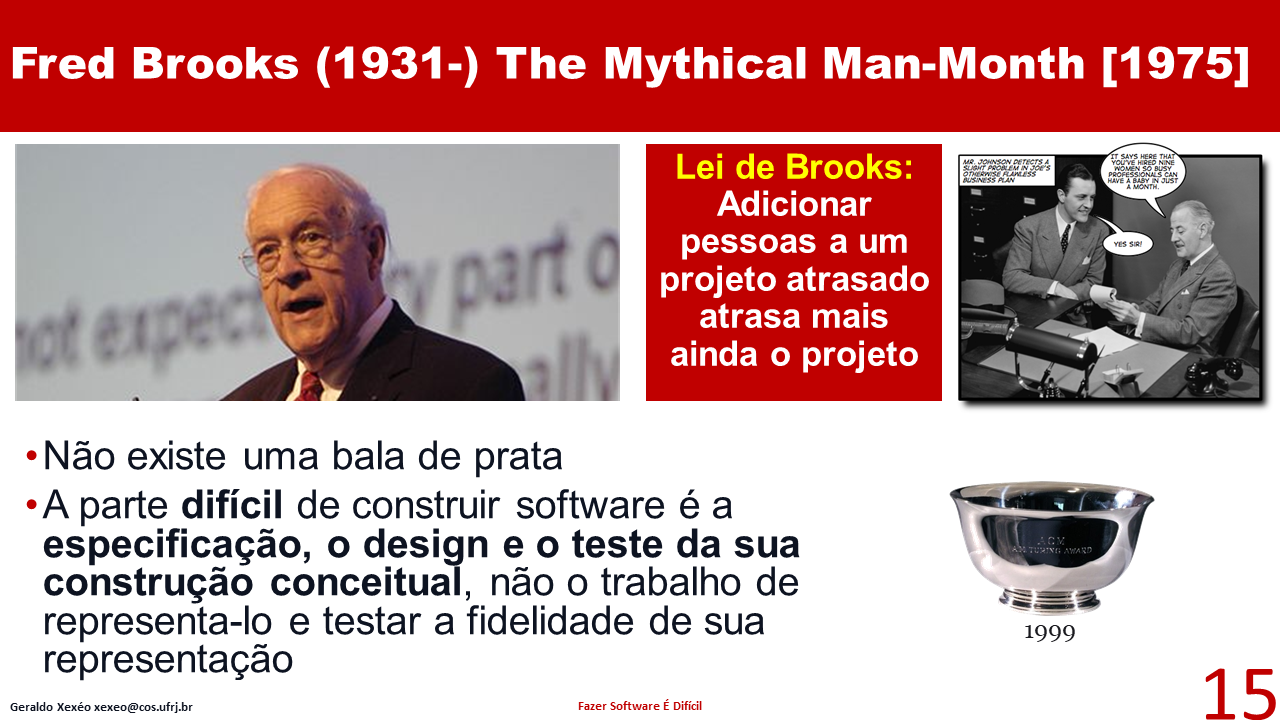
\includegraphics[width=\tam\linewidth]{imagens/manmonth.png}
    \caption{Um slide com um formato diferente}
    \label{fig:man}
\end{figure}


Os slides não devem ser exagerados, nem em texto, nem em decoração, porém um ou outro slide pode ser mais divertido, ou mais pesado em texto.

Em um slide com fórmulas, como o da Figura \ref{fig:formulas}, elas devem aparecer uma a uma se estiverem sendo calculadas. Se for apenas um comentário sobre a complexidade das fórmulas, que você deseje passar por cima em busca de uma explicação mais fácil, elas podem aparecer todas de uma vez.

\begin{figure}[hbt]
    \centering
    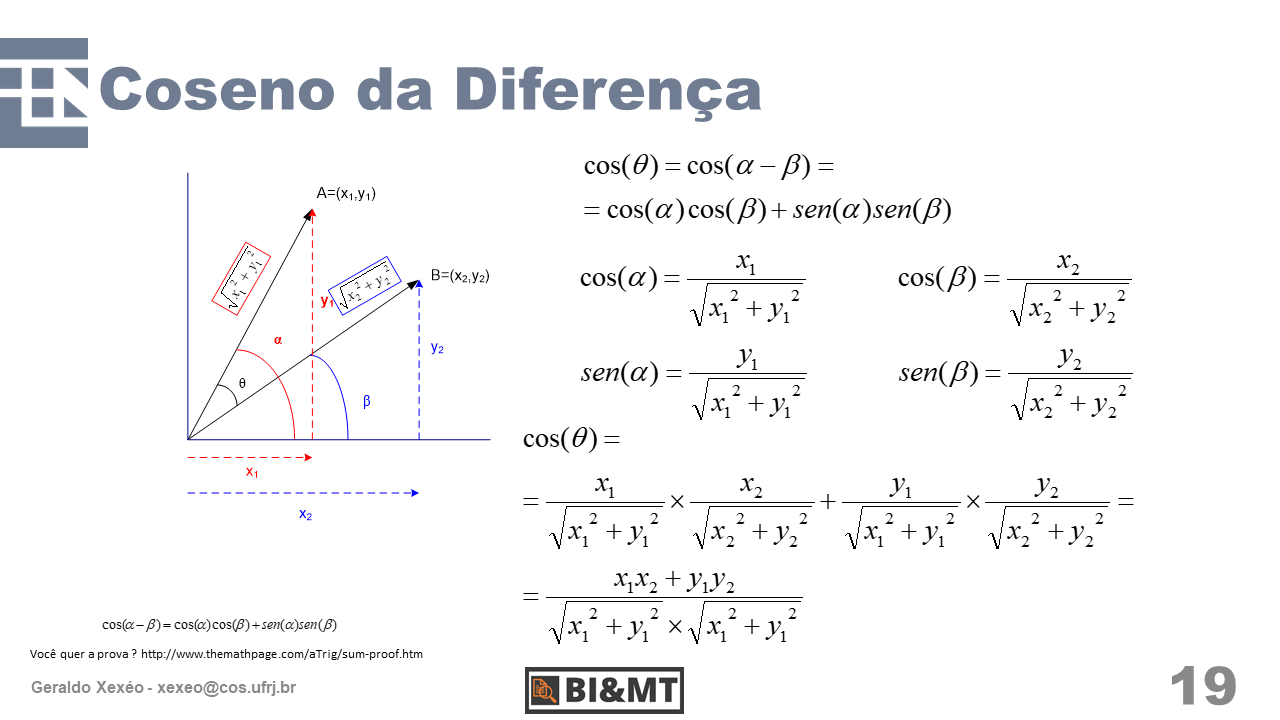
\includegraphics[width=\tam\linewidth]{imagens/desenhoeformulas.png}
    \caption{Desenho e fórmulas em um slide, que possui o logo do laboratório ligado ao curso e um logo que foi criado para identificar o curso em 3 lugares: Moodle, Whatsapp e GitHub.}
    \label{fig:formulas}
\end{figure}

\subsection{Que slides ter}

Os seguintes slides são recomendados para uma boa pontuação:
\begin{outline}
\1 Título da aula, como na Figura \ref{fig:titulo};
\2 Deve identificar candidato e ser feito como se fosse da instituição que faz o concurso;
\1 Objetivo da aula;
\1 Revisão do que é necessário para entender a aula;
\2 Contextualizando no curso
\1 Habilidades específicas que serão aprendidas;
\1 Agenda (ou Sumário);
\2 A agenda ou sumário divide a aula em seções;
\1 Um slide de título para cada seção;
\2 Pode ser o slide da agenda colocando ênfase na seção atual, como na Figura \ref{fig:meio};
\1 Slides de conteúdo;
\2 Não esqueça de uma motivação quando necessário;
\2 Não esqueça do contexto histórico do que está sendo ensinado;
\2 Não esqueça de definições
\1 Pelo menos um slide com um exercício
\2 Passar uma atividade de aprendizagem pós aula também é interessante, mesmo que ela nunca seja feita;
\1 Slide ``o que vimos hoje''
\2 Esse slide, ou slides, devem fechar a aula. Se necessário, por estar sobrando tempo, indique que agora, para reforçar, serão feitos ou discutidos exercícios, e siga por esse caminho até o fim do tempo;
\1 Referências bibliográficas;
\1 \textit{Preview} da próxima aula
\end{outline}

\begin{figure}[ht]
    \centering
    
\includegraphics[width=\tam\linewidth]{imagens/capa.png}
    \caption{Um slide de título.}
    \label{fig:titulo}
\end{figure}

Também é possível apresentar um slide de exercício no meio da aula. Nesse momento você deve ``quebrar a quarta parede'' e falar algo como ``normalmente eu daria 5 minutos e corrigiria o exercício, como vou fazer agora''.

Outra boa sugestão é ter um slide, no início, que leve a pensar sobre o conteúdo da aula. Esse slide pode mostrar um problema real onde a técnica poderia ser aplicada, sendo algo do tipo ``como vocês fariam para fazer x?''. Isso seria adequado para uma aula onde se ensina o método PERT/CPM para calcular prazos de um projeto. Já em uma aula de programação inicial, que vai usar exemplos numéricos, poderia ser proposto um problema numérico, como achar números primos.

Ao mostrar um problema é interessante mostrar como ele pode se complicar. Ao mostrar um método de fazer algo que suplantou outro anterior, é interessante mostrar os problemas que o anterior tinha. Deve haver cuidado, porém, na estimativa de tempo, o contexto histórico deve ser limitado a motivação. Se começar do início de tudo, você acabará tendo menos tempo para falar do assunto que deve abordar e poderá perder pontos.

\begin{figure}[hb]
    \centering
    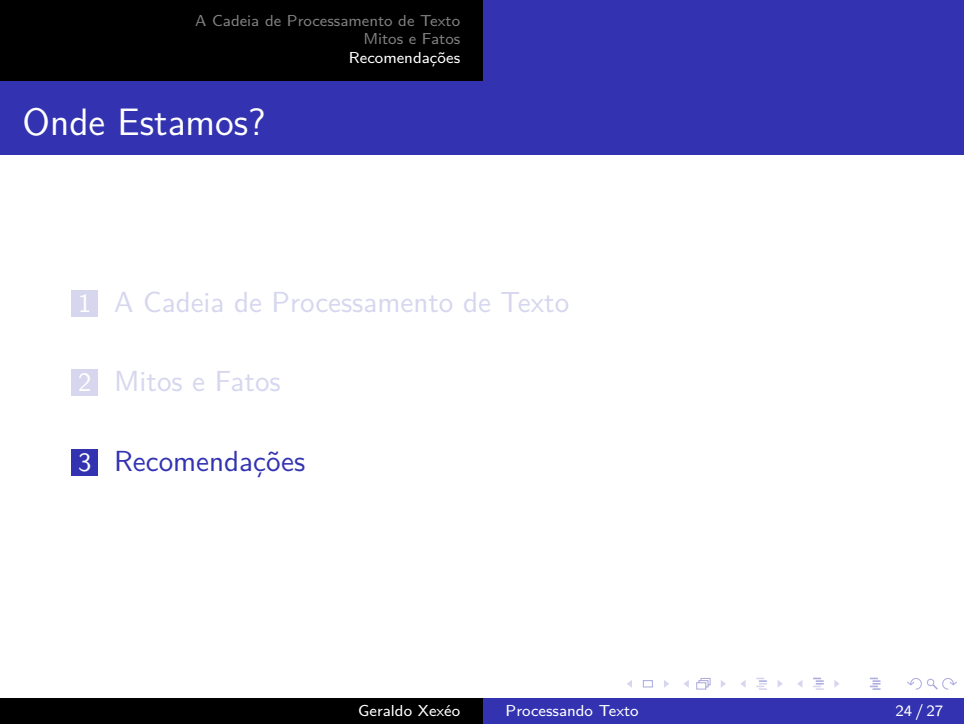
\includegraphics[width=\tam\linewidth]{imagens/agendadomeio.png}
    \caption{Um slide mostrando a parte que será falada da agenda, com as outras partes acinzentadas. Criada usando o \LaTeX\  e o \texttt{beamer}.}
    \label{fig:meio}
\end{figure}

Eu agora também crio mais um slide, que fala sobre a metodologia da aula, e o tamanho da aula em slides e em tempo, como na Figura \ref{fig:metodologia}. Esse slide também mostra como símbolos podem ser usados para passar mensagens. Julgo ser  uma boa ideia mostrar isso também, inclusive porque não é uma prática comum entre os professores e pode surpreender positivamente.

\begin{figure}[htb]
    \centering
    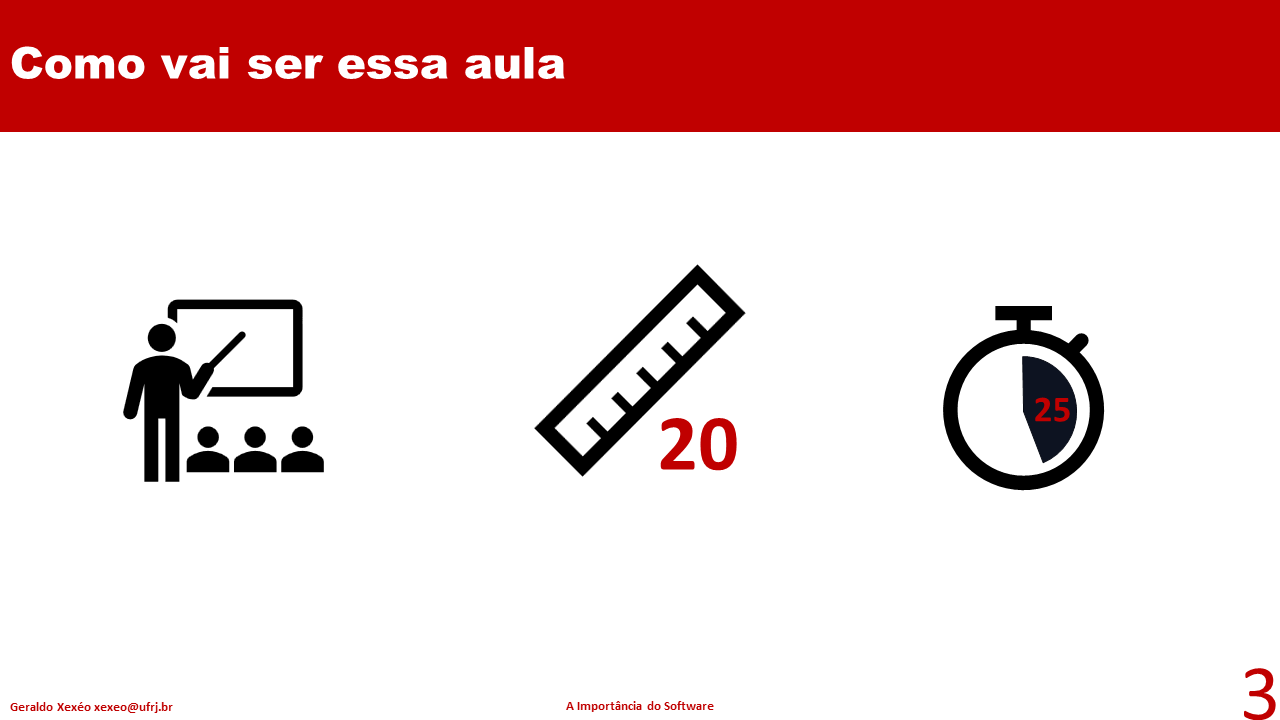
\includegraphics[width=\tam\linewidth]{imagens/metodologia.png}
    \caption{Slide informando o aluno como vai ser a aula.}
    \label{fig:metodologia}
\end{figure}


Em geral, qualquer prática didática adotada ativamente na aula vai ajudar a sua organização e, ao mesmo tempo, diminuir seu nervosismo. Outra vantagem é que vai facilitar a compreensão da banca não só do que está acontecendo na sua aula, mas principalmente porque você escolheu dar a aula dessa forma.

Como adicional, um slide final sobre você. Hoje, todas as minhas aulas terminam com o slide da Figura \ref{fig:fim}. Isso pode ser usado sempre para falar algo como ``quem quiser me contatar para tirar dúvidas...''.

\begin{figure}[h]
    \centering
    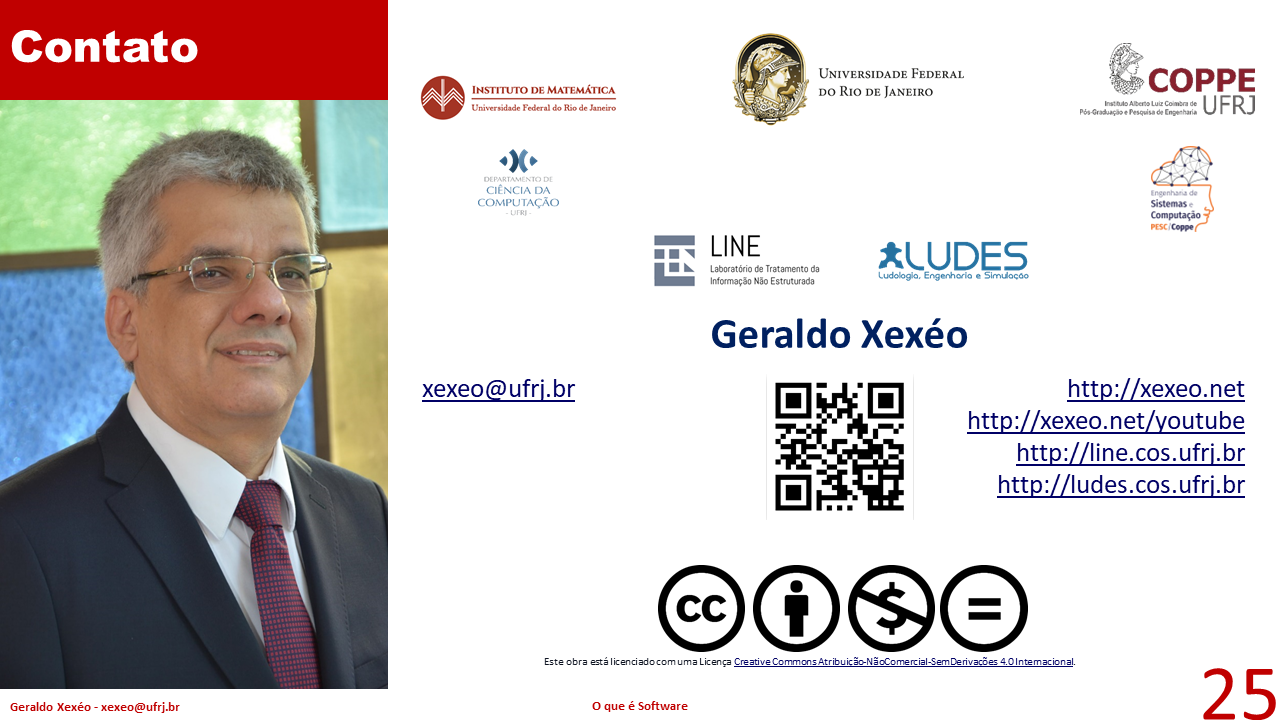
\includegraphics[width=\tam\linewidth]{imagens/fim.png}
    \caption{Um slide de contato.}
    \label{fig:fim}
\end{figure}

Forneça todas as referências, e indique a propriedade intelectual de tudo. Prefira imagens de domínio público ou com licenças amplas, como \textit{Creative Commons}.

\section{Material adicional}

Você deve entregar para a banca, impresso, se possível, um material adicional. Normalmente esse material adicional não está descrito no edital, porém ele é parte esperada de uma aula. Os candidatos que entregam isso já partem com vantagem.

O principal material adicional que considero obrigatório é o \textbf{plano de aula}. Existem muitos modelos na Web, mas um bom plano inclui:
\begin{outline}
\1 pré-requisitos;
\1 conteúdo da aula;
\1 objetivos gerais e específicos da aula;
\1 habilidades que o aluno deverá adquirir;
\2 Se possível usando a taxonomia revisada de Bloom
\1 metodologia;
\1 recursos didáticos necessários;
\1 forma de avaliação, e
\1 referências.
\end{outline}

Outros materiais possíveis são:
\begin{outline}
\1 lista de exercícios;
\1 leituras adicionais, na forma de capítulos ou artigos;
\end{outline}

Além de entregar o material, você deve mostrar em um slide onde podem ser encontrados na rede, por exemplo em um Moodle, ou no GitHub.

Eu recomendo entregar pelo menos uma lista de exercícios além do plano de aula. O resto pode ficar referenciado no seu falso Moodle, e ser mostrado em um slide para a ``turma''.


\section{Dicas para a aula}

Como dito no início, a prova de aula é quase um teatro. Quanto mais próximo você for de uma aula bem dada, dentro de um contexto imaginário de um curso bem construído, mais pontos você fará. Além disso, se conseguir quem entre os candidatos e candidatas que apresentam o contexto de melhor forma, suas chances de estar no topo da classificação aumentam.

Durante a aula, a preocupação com o uso do português é essencial. Erros de português não só prejudicam a nota, mas também desviam a atenção da banca, tendo um efeito prejudicial duplo. Outro problema semelhante é o uso de cacoetes de linguagem, como as palavras tipo, coisa, expressões como ``se pá'', e o gerundismo. Uma aula com conteúdo brilhante pode ser considerada  uma prática medíocre em função dos defeitos de fala e apresentação que podem ser causados pela falta de experiência, por vícios de linguagem ou por nervosismo.

Treine a aula buscando principalmente fluência e ter a ideia correta do tempo. Não é necessário decorá-la. A intenção do treino é melhorar a sua fluência, dicção, perceber o que pode explicar a mais e a menos.

Eu acredito que a aula deve ser dada \textbf{realmente} como a pessoa daria para a turma, isso significa que pode fazer brincadeiras ocasionais e ser informal em parte da aula. Porém, como é, na verdade, uma banca, não deve exagerar nas brincadeiras ou fazer delas o tom da aula. É bom ter algumas brincadeiras preparadas. Uma dose de sinceridade também pode ser útil, como dizer que quando era aluno achava o assunto muito difícil e que tentaria ser mais claro para os alunos que seus professores foram para você.

É interessante introduzir curiosidades. Eu, por exemplo, ao dar a aula de Casos de Uso, sempre falo para que os alunos não desenhem o ator sendo assaltado, isto é, com os braços para cima. Também sempre cito se um autor de algo que estou apresentando ganhou algum prêmio por isso, principalmente o prêmio Turing.

Não dê a matéria sem contexto. Existem dois contextos, um é o do curso, fictício ou existente, onde cabe a aula. O candidato deve, por exemplo, mostrar algo que já foi ensinado e está sendo usado na aula que está sendo dado. O outro é o contexto da própria matéria. Quem criou, inventou, que prêmios ganhou, qual foi a motivação original, questões de mercado, qual a importância do assunto, onde é usado.

Procure pelo menos um exemplo real de uso, algo que possa contar, se possível uma experiência pessoal.

\subsection{Como apresentar a aula}

Você deve falar sempre de frente e olhando para a banca, nunca falar de frente para os slides ou para o quadro, ou olhando para a tela do computador. Se tiver que usar o quadro, ou se virar, fale algo, então escreva ou desenhe de costas, em silêncio, e depois fale de novo.

No caso de aula remota coloque a câmera sobre a tela onde estão as transparências.

Mantenha um ritmo de fala, fale para fora, de preferência mais para alto, porém sem berrar. Professores sabem qual o seu tom na aula e devem se aproveitar desse conhecimento.

Não se mexa muito, nem pouco, e use os movimentos a seu favor.  Use as mãos e braços para indicar e para fazer sinais que façam sentido na aula. Por exemplo, se estiver falando de uma mensagem passando de um lugar para o outro, pode fazer um movimento de transferência com as mãos. Não fique caminhando pela sala, a não ser que tenha um objetivo específico, como distribuir um exercício, e faça esforço para não cruzar na frente do projetor, criando sombras na tela.

Sei que esses conselhos são difíceis. Mas lembre-se, não adianta treinar para ser um robô. A banca procura professores que deem aula de maneira natural.


Não leia os slides. Eles devem ser uma referência de posicionamento e continuidade da aula. Eles sintetizam o que deve ser dito. Use figuras, mas não dê uma aula como as palestras ``da moda'', só com imagens inspiradoras do assunto, o slide deve conter informação para poder guiar uma revisão ou um estudo mais aprofundado.

Muito cuidado com posicionamentos ideológicos, e certamente não faça piadas ou comentários de qualquer cunho depreciativo, ou preconceituoso.


Se vai falar nome de pesquisadores estrangeiros, e deve fazê-lo para falar de autores, procure a pronúncia correta na rede. De forma aproximada, Djkstra se fala dáistra, Huizinga se fala Raizingá, Marie Curie se fala Marrí Currí. Se for muito difícil, ou incomum usarem o nome correto no Brasil, chame atenção ao fato como chamaria atenção de uma turma, diga que foi pesquisar, etc. Novamente, use curiosidades para tornar a aula mais interessante, como ``Aliás, o nome original de Marie Curie era Maria Salomea Sk\l odowska, pronunciado praticamente como se lê em português, como o ``w'' com som de ``v''''.

\subsection{Pecados}

Com o nervosismo, muitas vezes são cometidos alguns ``pecados'' que incomodam muito a banca, como:
\begin{outline}
\1 errar o português;
\1 pigarrear seguidamente para tentar limpar a voz, ou outras formas de limpar a garganta;
\2 leve uma garrafa de água para dar aula;
\3 cuidado para também não exagerar no tempo em que toma um gole ou na quantidade de água;
\1 repetir palavras, como ``ok'', ``tá'' a todo momento;
\1 tossir sem proteger a boca;
\2 proteja com o braço de preferência;
\2 no caso de aula remota por vídeo, desligue o microfone;
\1 se coçar demais, coçar o nariz, morder ou roer as unhas ao pensar;
\1 qualquer ato não higiênico ou mal educado em geral.
\end{outline}

A desorganização também é um ``pecado'' que é mal-visto pela banca. Você deve chegar pronto para a aula, deve conhecer o software que vai usar e, se possível, deve estar disponível no local antes do horário para preparar o seu material.





\subsubsection{Pecados do português}

A seguir apresentamos alguns exemplos de português que ``doem no ouvido'' da banca.
\begin{outline}
\1 Cuidado com o uso do verbo haver:
\2 Como em ``\textbf{Há} muitos anos, \textbf{havia} sardinhas na Baía da Guanabara''.
\1 Advérbios não variam em número ou gênero.
\2 ``As esposas estavam meio chateadas porque os maridos estavam meio bêbados''.
\1 Como sujeito de verbo se usa ``eu'' e nunca ``mim''. Para eu fazer, para eu comprar. Cuidado ao dizer ``para mim'' e depois  completar a ideia com verbo, o que leva ao erro.
\1 Cuidado com os cacófatos, como ``O menor nun\textbf{ca} \textbf{ga}nha do maior''
\end{outline}

\section{Considerações especiais}

É possível, e até importante,  examinar o material didático dos membros da banca. Deve se ter cuidado ao usar como referência ou pegar pedaços diretamente deles, e só fazê-lo se previamente autorizado, por condições do material, e fazendo a citação correta.

A aula propriamente dita deve ser toda sua. Você pode se inspirar para ver os tópicos que a banca acha importante na agenda, a bibliografia, e pode também usar imagens de livros que os professores da banca também usam. Ao fazer isso, porém, deve ter muito cuidado com o plágio.

\section{Regras mais importantes}

\begin{enumerate}
\item Use corretamente o português.
\item Pronuncie corretamente as palavras em outras línguas.
\item Verifique a correção e atualização do conteúdo da aula.
\item Organize-se.
\item Tenha atenção as práticas didáticas.
\item Treine para evitar o nervosismo.
\item Se divirta dando a aula.
\end{enumerate}

\section{Colabore!}

Este texto foi escrito como uma conversa com uma pessoa da qual não é necessário conhecer o gênero. Esta pessoa é chamada de você, como se faz no Rio de Janeiro. Ele foi revisado para ser indiferente ao gênero de todas as formas possíveis quando lido, não fazendo também suposições sobre o gênero da pessoa que se candidata à vaga. Se você julga que em alguma parte do texto esta intenção se perde, por favor se comunique comigo.

Se você tem outras dicas, por favor mande uma mensagem para mim.



\section{Licença}

Este texto é distribuído com uma licença Creative Commons - Atribuição - NãoComercial - Compartilha Igual 4.0 Internacional.


Você tem o direito de:
\begin{itemize}
\item \textbf{Compartilhar} -- copiar e distribuir o material em qualquer suporte ou formato.
\item \textbf{Adaptar} -- remixar, transformar, e criar a partir do material.
\end{itemize}

De acordo com os termos seguintes:
\begin{itemize}
\item \textbf{Atribuição} -- Você deve dar o crédito apropriado, prover um link para a licença e indicar se mudanças foram feitas. Você deve fazê-lo em qualquer circunstância razoável, mas de nenhuma maneira que sugira que o licenciante apoia você ou o seu uso.
\item \textbf{NãoComercial} --Você não pode usar o material para fins comerciais.
\item \textbf{CompartilhaIgual} -- Se você remixar, transformar, ou criar a partir do material, tem de distribuir as suas contribuições sob a mesma licença que o original.
\item \textbf{Sem restrições adicionais} -- Você não pode aplicar termos jurídicos ou medidas de caráter tecnológico que restrinjam legalmente outros de fazerem algo que a licença permita.
\end{itemize}

Mais informações podem ser encontradas em \url{https://creativecommons.org/licenses/by-nc-sa/4.0/deed.pt_BR}
\end{document}
